%!TEX root = ../masters_thesis.tex

\section{Application} % (fold)
\label{sec:application}

HistoGlobe is a Web-based Historical Geographic Information System. The Data model and the conceptual model of the user interface were introduced in the first two sections of this chapter. This section introduces the underlying database model, a specific implementation of the data model, and the computational model that translates between the conceptual model and the database model of the system.

The first part provides an overview about the architecture of the system in section \ref{sub:system_architecture}.
% ... bla bla bla, the rest comes last
% problems
% - backward change: all HG Operations and Edit Operations are inversible :)
% - support uncertainty

% ------------------------------------------------------------------------------
\subsection{System Architecture} % (fold)
\label{sub:system_architecture}

HistoGlobe uses a classical client-server architecture of a Web-based information system. The user opens the application and interacts with it through the user interface in a Web browser, the \emph{client} side of the system. The Web \emph{server} is a remote computer that hosts the database and the middleware. The user interacts with the interface, the client-side application sends a request to the Web server for new data. The middleware checks the request and queries the necessary data from the database. It transforms the data and sends it back to the client. The interface shows the new information.

\begin{figure}[H]
  \vspace{1em}
  \centering
  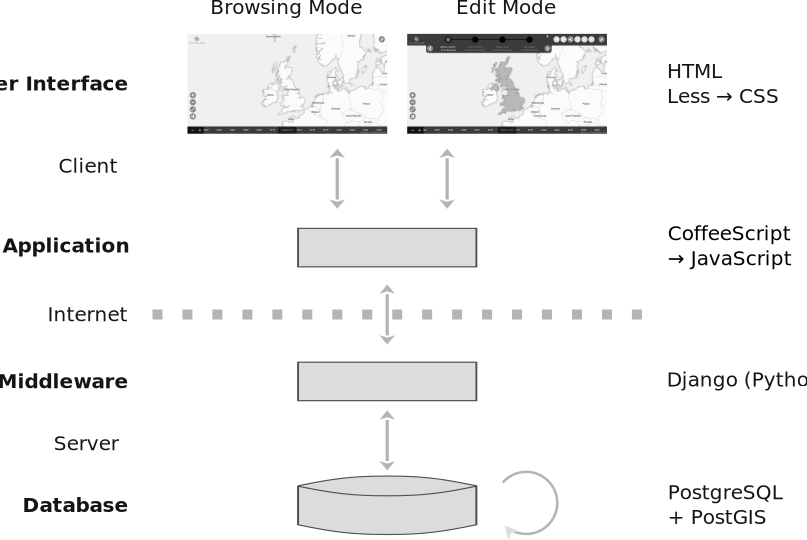
\includegraphics[width=0.7\textwidth]{graphics/development/system_architecture}
  \caption{The system architecture of HistoGlobe}
  \label{fig:system_architecture}
\end{figure}

This clear separation between the data, the application and the user interaction in this chapter and in the system follows directly from the \emph{model-view-controller} pattern: One part can be changed independently from the others parts: if the 2D map is replaced by a 3D globe, only the view changes, but the middleware and the database can stay untouched. Likewise, the implementation of a new database technology has no consequences to the view.

% subsection system_architecture (end)

% ------------------------------------------------------------------------------
\subsection{Database Model} % (fold)
\label{sub:database_model}

database model

\begin{compactenum}
  \item The \emph{name} of the Hivent.
  \item A textual \emph{description} of the topic of the Hivent.
  \item The point in time, identified by the Hivent \emph{date}.
  \item The Hivent \emph{location}.
  \item The \emph{historical changes} resulting from the Hivent.
\end{compactenum}


           Hivent
             |
             m
       HistoricalChange
             |
             m
  |-------AreaChange-----|
  |         |  |         |
  |         m  m         |
  |     |---Area---|     |
  m     m          m     m
AreaTerritory      AreaName

no transaction time, only valid / event time
only world time is regarded, not database time.

view

get\_all
save\_operation

% subsection database_model (end)


% ------------------------------------------------------------------------------
\subsection{Computational Model} % (fold)
\label{sub:computational_model}

Class diagram

HistoGlobe

SpatialDisplay -> Map

TimeController  <-> Timeline
                <-> NowMarker

HiventController                AreaController <->  AreasOnMap
HiventHandle                    AreaHandle
Hivent
HistoricalChange    AreaChange  Area
                                AreaName            AreaNameLayerOnMap
                                AreaTerritory       AreaTerritoryLayerOnMap

DatabaseInterface

EditMode -> EditOperation -> EditOperationStep
NewTerritoryTool* NewNameTool NewHiventBox
WorkflowWindow

HistoGraph

LabelManager*

important little utils
  Button, ButtonArea
  NumberInput, TextInput, TextInputArea
  Title
  Watermark
  DoublyLinkedList
  WithinTree
  Geometry -> Polypolygon -> Polygon -> Polyline -> Point

% - - - - - - - - - - - - - - - - - - - - - - - - - - - - - - - - - - - - - - -
\paragraph{Reduction to HG Operations} % (fold)
\label{par:reduction_to_hg_operations}

The conceptual model promotes six Edit Operations (see section \ref{sub:edit_operations}) that humans can understand.
The underlying data model is based on five HG Operations (see section \ref{tab:historical_geographic_operations}) that can model all evolutionary changes to countries in time and space. The task for the computational model of HistoGlobe is to translate between both operation sets.

% wording:
% UNI of "[old]"  to    "new"
% INC of "[old]"  into  "pres"
% SEP of "old"    into  "[new]"
% SEC of "[new]"  from  "pres"
% NCH of "pres"

Each Edit Operation will internally be expressed by a set of Historical Geographic Operations that describe the change on a low level. Depending on the input of the user in the Edit Operation steps, there are different possibilities. They are introduced in table \ref{tab:editoperations_to_hg_operations}.

\begin{center}
\begin{longtable}{m{1.2cm} m{0.95cm} m{0.95cm} m{0.95cm} m{6.0cm} m{2.3cm}}
  \toprule

  \pbox{1.2cm}{EditOp.\\(case)} &
  \pbox{0.95cm}{old\\Areas\\[-0.8em]} &
  \pbox{0.95cm}{update\\Areas\\[-0.8em]} &
  \pbox{0.95cm}{new\\Areas\\[-0.8em]} &
  expression by HG Operations \protect\footnotemark &
  visualization \\
  \midrule
  \endhead

  % TODO: introduce T as territory that is used like a temporary Area with exactly that territoy
  % CREATE

  \multirow{9}{*}{\texttt{CRE} (1)} &
  \multicolumn{4}{p{10cm}}{
    Area $B_1$ is created with territory $T$. The part of $T$ that is on previously unclaimed land ($T_\Omega$) is seceded as $B_1$ from $\Omega$.
    If $T_\Omega$ is empty, then $B_1$ is initialized with an empty territory.
    The rest of $T$ covers some Areas $A_p$ partially and some Areas $A_f$ fully.
    For each $A_p$, the covered territory $T_p$ is seceded and incorporated into $B_1$.
    Each $A_f$ is completely incorporated into $B_1$.
  } &
  \multirow{9}{*}{
    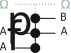
\includegraphics[width=2.5cm]{graphics/development/edit_to_hg_operations/CRE_to_SEC+UNI}
  } \\

  &
  $n_f$ &
  $n_p$ &
  $1$ &
  \pbox{6.0cm}{
    ~\\
    \texttt{SEC} of $B_1$ from $\Omega$ \\
    \texttt{SEC} of $T_p$ from $A_p$, \texttt{INC} of $T_p$ into $B_1$ \\
    \texttt{INC} of $A_f$ into $B_1$
  } &
  \\

  % MERGE
  \midrule
  \multirow{3}{*}{\texttt{MRG} (1)} &
  \multicolumn{4}{p{10cm}}{
    Multiple Areas $A_i$ are unified to $B_1$. The new Area receives a new name distinct from all the names of $A_i$.
  } &
  \multirow{3}{*}{
    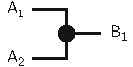
\includegraphics[width=2.5cm]{graphics/development/edit_to_hg_operations/MRG_to_UNI}
  } \\
  &
  $n \geq 2$ &
  $0$ &
  $1$ &
  \pbox{6.0cm}{
    ~\\
    \texttt{UNI} of $\forall A_i$ to $B_1$
  } &
  \\

  \midrule
  \multirow{4}{*}{\texttt{MRG} (2)} &
  \multicolumn{4}{p{10cm}}{
    Multiple Areas $A_i$ are unified, the resulting Area reuses the short and formal name of one of the old Areas ($A_p$) and therefore preserves it. The remaining Areas $A_i$ are incorporated into $A_p$.
  } &
  \multirow{4}{*}{
    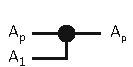
\includegraphics[width=2.5cm]{graphics/development/edit_to_hg_operations/MRG_to_INC}
  } \\
  &
  $n \geq 1$ &
  $1$ &
  $1$ &
  \pbox{6.0cm}{
    ~\\
    \texttt{INC} of $\forall A_i$ into $A_p$
  } &
  \\

  \midrule
  \multirow{4}{*}{\texttt{MRG} (3)} &
  \multicolumn{4}{p{10cm}}{
    The same as the previous case, just that $A_p$ receives a new short name and therefore an additional name change is required.
  } &
  \multirow{4}{*}{
    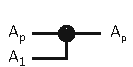
\includegraphics[width=2.5cm]{graphics/development/edit_to_hg_operations/MRG_to_INC+NCH}
  } \\
  &
  $n \geq 1$ &
  $1$ &
  $1$ &
  \pbox{6.0cm}{
    ~\\
    \texttt{INC} of $\forall A_i$ into $A_p$ \\
    \texttt{NCH} of $A_p$
  } &
  \\

  % DISSOLVE

  \midrule
  \multirow{4}{*}{\texttt{DIS} (1)} &
  \multicolumn{4}{p{10cm}}{
    Separate one Area $A_1$ into multiple new Areas $B_i$ and define a territory and name for each of them. Each name is distinct from the name of the old Area.
  } &
  \multirow{4}{*}{
    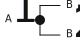
\includegraphics[width=2.5cm]{graphics/development/edit_to_hg_operations/DIS_to_SEP}
  } \\
  &
  $1$ &
  $0$ &
  $n \geq 2$ &
  \pbox{6.0cm}{
    ~\\
    \texttt{SEP} of $A_1$ into $\forall B_i$
  } &
  \\

  \midrule
  \multirow{5}{*}{\texttt{DIS} (2)} &
  \multicolumn{4}{p{10cm}}{
    Separate multiple Areas $B_1$ from one initial Area $A_p$ and define a territory and name for each of them. One of the separated Areas has the same short and formal name as $A_p$, so it continues its identity and preserves the Area. The remaining new Areas secede from $A_p$.
  } &
  \multirow{5}{*}{
    
\includegraphics[width=2.5cm]{graphics/development/edit_to_hg_operations/DIS_to_SEC}
  } \\
  &
  $1$ &
  $1$ &
  $n \geq 1$ &
  \pbox{6.0cm}{
    ~\\
    \texttt{SEC} of $\forall B_i$ from $A_p$
  } &
  \\

  \midrule
  \multirow{4}{*}{\texttt{DIS} (3)} &
  \multicolumn{4}{p{10cm}}{
    The same as the previous case, just that $A_p$ receives a new short name and therefore an additional name change is required.
  } &
  \multirow{4}{*}{
    
\includegraphics[width=2.5cm]{graphics/development/edit_to_hg_operations/DIS_to_SEC+NCH}
  } \\
  &
  $1$ &
  $1$ &
  $n \geq 1$ &
  \pbox{6.0cm}{
    ~\\
    \texttt{SEC} of $\forall B_i$ from $A_p$  \\
    \texttt{NCH} of $A_p$
  } &
  \\

  % CHANGE BORDER

  \midrule
  \multirow{10}{*}{\texttt{CHB} (1)} &
  \multicolumn{4}{p{10cm}}{
    One existing Area $A_1$ is selected and its territory changes. Relative to the old territory some parts of the territory expanded ($T_e$) and some withdrew ($T_w$).
    The part of $T_e$ that expanded into unclaimed land ($T_\Omega \in T_e$) is seceded from $\Omega$ and incorporated into $A_1$.
    The Areas $A_f$ fully covered by $T_e$ are incorporated into $A_1$,
    the Areas $A_p$ partially covered by $T_e$ secede this territory $T_p \in T_e$ to $A_1$.
    $T_w$ will be incorporated into $\Omega$, resulting in unclaimed land.
  } &
  \multirow{10}{*}{
    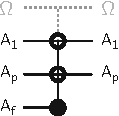
\includegraphics[width=2.5cm]{graphics/development/edit_to_hg_operations/CHB_to_SEC+INC_omega}
  } \\
  &
  $n_f$ &
  $1+n_p$ &
  $0$ &
  \pbox{6.0cm}{
    ~\\
    \texttt{SEC} of $T_\Omega$ from $\Omega$,
    \texttt{INC} of $T_\Omega$ into $A_1$ \\
    \texttt{SEC} of $T_p$ from $A_p$,
    \texttt{INC} of $T_p$ into $B_1$ \\
    \texttt{INC} of $A_f$ into $B_1$ \\
    \texttt{SEC} of $T_w$ from $B_1$,
    \texttt{INC} of $T_w$ into $\Omega$
  } &
  \\

  \midrule
  \multirow{7}{*}{\texttt{CHB} (2)} &
  \multicolumn{4}{p{10cm}}{
    Two existing Areas $A_1$ and $A_2$ are selected and their common border changes. This results in a symmetrical change of territories, made up by two sets of territories: $T_2$ that previously belonged to $A_1$ and is now part of $A_2$ and $T_1$ for which the opposite is true. $T_2$ is seceded by $A_1$ and incorporated into $A_2$, the opposite happenes to $T_1$.
  } &
  \multirow{7}{*}{
    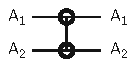
\includegraphics[width=2.5cm]{graphics/development/edit_to_hg_operations/CHB_to_SEC+INC}
  } \\
  &
  $0$ &
  $2$ &
  $0$ &
  \pbox{6.0cm}{
    ~\\
    \texttt{SEC} of $T_2$ from $A_1$,
    \texttt{INC} of $T_2$ into $A_2$ \\
    \texttt{SEC} of $T_1$ from $A_2$,
    \texttt{INC} of $T_1$ into $A_1$
  } &
  \\

  % RENAME

  \midrule
  \multirow{3}{*}{\texttt{REN} (1)} &
  \multicolumn{4}{p{10cm}}{
    One Area $A_1$ is selected and both its short and formal name is changed. Therefore, a new Area $B_1$ is created as a direct successor of $A_1$. This is a special case of a unification with only one Area.
  } &
  \multirow{3}{*}{
    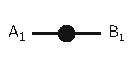
\includegraphics[width=2.5cm]{graphics/development/edit_to_hg_operations/REN_to_UNI}
  } \\
  &
  $1$ &
  $0$ &
  $1$ &
  \pbox{6.0cm}{
    \texttt{UNI} of $A_1$ to $B_1$
  } &
  \\

  \midrule
  \multirow{3}{*}{\texttt{REN} (2)} &
  \multicolumn{4}{p{10cm}}{
    One Area $A_1$ is selected and receives a new short name, but the formal name and therefore the identity is preserved. $A_1$ is updated.
  } &
  \multirow{3}{*}{
    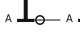
\includegraphics[width=2.5cm]{graphics/development/edit_to_hg_operations/REN_to_NCH}
  } \\
  &
  $0$ &
  $1$ &
  $0$ &
  \pbox{6.0cm}{
    \texttt{NCH} of $A_1$
  } &
  \\

  % CEASE

  \midrule
  \multirow{2}{*}{\texttt{CES} (1)} &
  \multicolumn{4}{p{10cm}}{
    One Area $A_1$ is selected and ceases by incorporating into the universe.
  } &
  \multirow{2}{*}{
    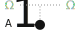
\includegraphics[width=2.5cm]{graphics/development/edit_to_hg_operations/CES_to_INC}
  } \\
  &
  $1$ &
  $0$ &
  $0$ &
  \pbox{6.0cm}{
    \texttt{INC} of $A_1$ into $\Omega$
  } &
  \\

  \bottomrule
\caption{Translation from Edit Operations to HG Operations}
\end{longtable}
\label{tab:editoperations_to_hg_operations}
\end{center}
\footnotetext{multiple HG Operations in one row happen exactly at the same time point, so they are combined}

% paragraph reduction_to_hg_operations (end)

% - - - - - - - - - - - - - - - - - - - - - - - - - - - - - - - - - - - - - - -
\paragraph{Functional description} % (fold)
\label{par:functional_description}

Each HG Operation can be described by a mathematical function. The following symbols are used in the equations:

\begin{addmargin}[1em]{0em}
\begin{tabbing}
  symbolxx \= description1xx \= description2 \kill
  $A$ \> set of old Areas that were active before the Historical Change \\
  $B$ \> set of new Areas that are created in the Historical Change \\
  $n:$ \> $n \in \mathbb{N}, n>0$ \> total number of old respectively new Areas \\
  $i:$ \> $i \in [\textbf{1} .. n]$ \> iterator for the current old respectively new Area \\
  $A_0/B_0$ \>    the first old respectively new Area ($i \geq 1 \Rightarrow$ not $A_i/B_i$~!) \\
  $A_i/B_i$ \>    the current old respectively new Area ($i \geq 1 \Rightarrow$ not $A_0/B_0$~!) \\
  $A_i^T/B_i^T$ \>the new territory of the current Area (a polypolygon) \\
  $A_i^N/B_i^N$ \>the new name of the current Area (short and formal name) \\
\end{tabbing}
\end{addmargin}

\vspace{-2.5em}
\begin{align*}
  (B_0)                       &= UNI([A_1 .. A_i .. A_n], B_0^N) \\
  (A_0)                       &= INC(A_0, [A_1 .. A_i .. A_n]) \\
  ([B_1 .. B_i .. B_n])       &= SEP(A_0, [[B_1^T, B_1^N] .. [B_i^T, B_i^N] .. [B_n^T, B_n^N]]) \\
  (A_0, [B_1 .. B_i .. B_n])  &= SEC(A_0, A_0^T, [[B_1^T, B_1^N] .. [B_i^T, B_i^N] .. [B_n^T, B_n^N]]) \\
  (A_0)                       &= NCH(A_0, A_0^N)
\end{align*}

% paragraph functional_description (end)

% - - - - - - - - - - - - - - - - - - - - - - - - - - - - - - - - - - - - - - -
\paragraph{Pseudocode description} % (fold)
\label{par:pseudocode_description}

of the HG operations in an object-oriented manner. The existance of a class \texttt{Area} is assumed. Each \texttt{Area} object has the following member variables: a \texttt{name}, a \texttt{territory} and a list of historical \texttt{predecessors} and \texttt{successors}. Single capital letter variables (\texttt{A}/\texttt{B}) denote arrays of \texttt{Area} objects. Variables with a capital letter followed by a number or lowercase letter (e.g. \texttt{B0}) are single \texttt{Area} objects.

\begin{minipage}[t]{0.47\textwidth}
\begin{lstlisting}[language=pseudocode,
  caption=Unification]
FUNCTION UNI(A, B0_name)
  # create new territory
  B0_territory = NEW Geometry # empty
  FOREACH Ai IN A
    B0_territory.union(Ai.territory)
  # create new area
  B0 = NEW Area(B0_name, B0_territory)
  # establish historical relationships
  FOREACH Ai IN A
    Ai.successors.add(B0)
    B0.predecessors.add(A1)
  # return new area
  RETURN B0
\end{lstlisting}
\end{minipage}    % N.B. the % is very important
\hspace{3.0em}    % N.B. this must go in this line, no blank lines !!!
\begin{minipage}[t]{0.47\textwidth}
\begin{lstlisting}[language=pseudocode,
  caption=Incorporation]
FUNCTION INC(A0, A)
  # update old area with new territory
  temp_terr = NEW Geometry # empty
  FOREACH Ai IN A
    temp_terr.union(Ai.territory)
  A0.territory = temp_terr
  # establish historical relationships
  FOREACH Ai IN A
    Ai.successor.add(A0)
    A0.predecessor.add(A1)
  # return new area
  RETURN A0
\end{lstlisting}
\end{minipage}

\begin{minipage}[t]{0.47\textwidth}
\begin{lstlisting}[language=pseudocode,
  caption=Separation]
FUNCTION SEP(A0, B_data)
  # create each new Area
  B = []
  FOREACH Bi_data in B_data
    B.add(NEW Area(
      Bi_data.name, Bi_data.territory)
    )
  # establish historical relationships
  FOREACH Bi IN B
    A0.successors.add(Bi)
    Bi.predecessors.add(A0)
  # return new areas
  RETURN B

\end{lstlisting}
\end{minipage}    % N.B. the % is very important
\hspace{3.5em}    % N.B. this must go in this line, no blank lines !!!
\begin{minipage}[t]{0.47\textwidth}
\begin{lstlisting}[language=pseudocode,
  caption=Secession]
FUNCTION SEC(A0, A_territory, B_data)
  # update old area with new territory
  A0.territory = A_territory
  # create each new Area
  B = []
  FOREACH Bi_data in B_data
    B.add(NEW Area(
      Bi_data.name, Bi_data.territory)
    )
  # establish historical relationships
  FOREACH Bi IN B
    A0.successors.add(Bi)
    Bi.predecessors.add(A0)
  # return old and new areas
  RETURN [A0, B]

\end{lstlisting}
\end{minipage}

\vspace{-1.5em}
\begin{minipage}[t]{0.47\textwidth}
\begin{lstlisting}[language=pseudocode,
  caption=Name Change]
FUNCTION NCH(A0, A_name)
  # update old area with new name
  A0.name = A_name
  # return updated area
  RETURN A0

\end{lstlisting}
\end{minipage}

% paragraph pseudocode_description (end)


\paragraph{Execute Historical Change} % (fold)
\label{par:execute_historical_change}

execute function for all operations the same

% - - - - - - - - - - - - - - - - - - - - - - - - - - - - - - - - - - - - - - -
\begin{lstlisting}[language=pseudocode,
  caption=class HGOperation]
## member variables
old_areas = []          # Area
new_areas = []          # Area
update_name = {
  area :          null  # Area
  old_name :      null  # AreaName
  new_name :      null  # AreaName
}
update_territory = {
  area :          null  # Area
  old_territory : null  # AreaTerritory
  new_territory : null  # AreaTerritory
}

## main function
FUNCTION execute(direction)

  # hide old areas
  FOREACH old_area IN old_areas
    IF direction IS 1 # forward change
      old_area.hide()
    ELSE              # backward change
      old_area.show()

  # show new areas
  FOREACH new_area IN new_areas
    IF direction IS 1 # forward change
      new_area.show()
    ELSE              # backward change
      new_area.hide()

  # check if the area name is updated
  IF update_name.area
    IF direction IS 1 # forward change
      update_name.area.name = new_name
    ELSE              # backward change
      update_name.area.name = old_name
    update_name.area.update()

  # check if the area territory is updated
  IF update_territory.area
    IF direction IS 1 # forward change
      update_territory.area.territory = new_territory
    ELSE              # backward change
      update_territory.area.territory = old_territory

\end{lstlisting}

% paragraph execute_historical_change (end)

HistoGraph
\begin{lstlisting}[language=pseudocode,
  caption=plotting Areas on the HistoGraph,
  label=lst:histograph_plot]
FUNCTION plot(reference_area, plot_start_date, plot_end_date)
  # plot the current Area
  # logic is omitted

  # recursively plot in historically backward direction
  FOREACH predecessor IN reference_area.predecessors
    IF predecessor.end_date >= plot_start_date
      plot(predecessor)

  # recursively plot in historically forward direction
  FOREACH successor IN reference_area.successors
    IF successor.start_date <= plot_end_date
      plot(successor)
\end{lstlisting}

store Hivents in DoublyLinkedList

% \begin{figure}[ht]
%   \centering
%   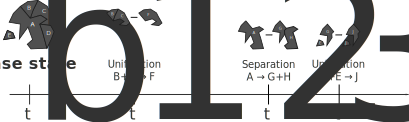
\includegraphics[width=0.8\textwidth]{graphics/basics/stdm/event-based_spatio-temporal_data_model}
%   \caption{The Event-Based Spatio-Temporal Data Model}
%   \label{fig:event-based_spatio-temporal_data_model}


A main problem is to maintain the integrity of the spatial topology when a new change gets inserted not at the end of the list. A simple example shows that problem: Given geo-object $X$ is part of the inital base configuration at change $t_b$. At a later change, e.g. $t_y$ $X$ gets replaced by object $Y$. If a new change that updates $X$ to $X'$ gets inserted before at time point $t_x < t_y$, then $t_y$ is not integer anymore, because object $X$ does not exist. That is why on insertion of a change, all succeeding changes have to be tested for integrity and it might be necessary to update later changes.


% subsection computational_model (end)

% section application (end)